%==============================================================================
% Sjabloon poster bachproef
%==============================================================================
% Gebaseerd op document class `a0poster' door Gerlinde Kettl en Matthias Weiser
% Aangepast voor gebruik aan HOGENT door Jens Buysse en Bert Van Vreckem

\documentclass[a0,portrait]{hogent-poster}

% Info over de opleiding
\course{Bachelorproef}
\studyprogramme{toegepaste informatica}
\academicyear{2024-2025}
\institution{Hogeschool Gent, Valentin Vaerwyckweg 1, 9000 Gent}

% Info over de bachelorproef
\title{De impact van mobiele netwerken op facilitair beheer: een vergelijkende studie van 4G en privaat 5G voor HOGENT}
%\subtitle{Ondertitel (eventueel)}
\author{Jan De Somviele}
\email{jan.desomviele@student.hogent.be}
\supervisor{Lena De Mol, Chantal Teerlinck}
\cosupervisor{Giselle Vercauteren (HOGENT)}

% Indien ingevuld, wordt deze informatie toegevoegd aan het einde van de
% abstract. Zet in commentaar als je dit niet wilt.
\specialisation{Systeem- en Netwerkbeheer}
\keywords{5G, 4G, gebouwbeheer}
\projectrepo{https://github.com/JanDeSomviele/Bachelorproef2025}

\begin{document}

\maketitle

\begin{abstract}
Dit onderzoek focust op de prestaties en betrouwbaarheid van 4G- en privaat 5G-netwerken m.b.t. gebouwbeheersystemen zoals verlichting en HVAC.
Via netwerkmetingen en functionele testen worden praktische implicaties en geschiktheid van mobiele netwerken binnen smart buildings bestudeerd.
\end{abstract}

\begin{multicols}{2} % This is how many columns your poster will be broken into, a portrait poster is generally split into 2 columns

\section{Introductie}

Deze bachelorproef onderzocht hoe 4G en privaat 5G-netwerken presteren binnen een gebouwbeheersysteem (GBS), met toepassingen zoals verlichting en HVAC. De centrale onderzoeksvraag luidde: \textit{Wat is het verschil tussen 4G en privaat 5G in verband met prestaties en betrouwbaarheid van toepassingen binnen een GBS?}



\section{Experimenten}
De experimenten om de netwerkeigenschappen te meten gebeurden in een testopstelling met twee configuraties. Beide hebben een pc bekabeld verbonden met een router die wisselend wifi, 4G of privaat 5G levert. Een meetnode simuleert de aansturing van het GBS. In opstelling A fungeert een Raspberry Pi als meetnode. In opstelling B is dit een Philips Hue Bridge gecombineerd met een Philips Hue smartlight.

\begin{center}
    \captionsetup{type=figure}
    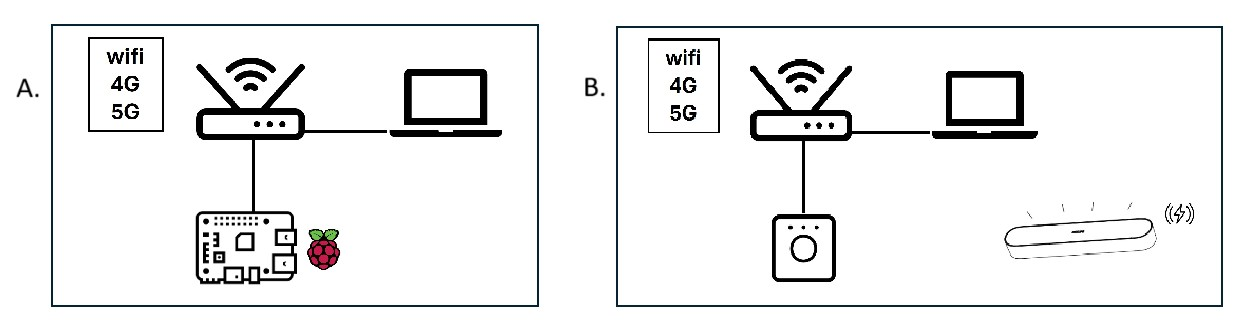
\includegraphics[width=0.45\textwidth]{../graphics/beideOpstellingen.jpg}
    \captionof{figure}{Opstelling A met Raspberry Pi meetnode en Opstelling B met Philips Hue Bridge en smartlight}
\end{center}


\begin{multicols}{2}
\subsection*{Latency}

Latency, gemeten als round-trip-time (RTT),is de tijd die een datapakket nodig heeft om heen en terug te reizen tussen twee punten. Met het commando ’ping -c 250’ naar een extern IP werd gekeken naar de snelheid en stabiliteit van de netwerken. Wifi had de laagste gemiddelde latency (13,27 ms) gevolgd door 4G (18,17 ms). De gemiddelde latency van 5G was hoger: ondanks een lage minimumwaarde (10,85 ms) waren er ook grote pieken tot 230,92 ms. Dit kan wijzen op fluctuaties in de testomgeving of instabiliteit van het privaat 5G-netwerk.
\subsection*{Jitter}

Jitter geeft de variatie in vertraging tussen opeenvolgende datapakketten weer. Dit is belangrijk voor betrouwbare real-time toepassingen zoals HVAC en lichtsturing. Met iperf3 werden per netwerk drie UDP-tests uitgevoerd (1, 5 en 50 Mbit/s) waarbij jitter werd gemeten. Bij 1 Mbit/s had wifi de hoogste jitter (0,799 ms), terwijl 4G en 5G stabieler waren. Bij hogere snelheden daalden de jitterwaarden en stabiliseerden alle netwerken rond 0,15–0,20 ms.\newline
\end{multicols}
\begin{center}
    \captionsetup{type=figure}
    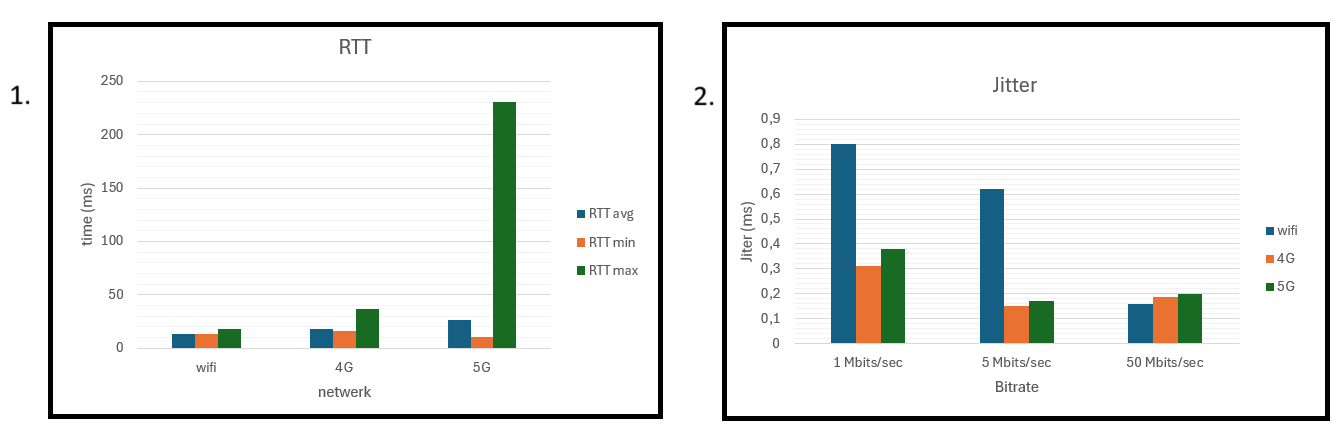
\includegraphics[width=0.45\textwidth]{../graphics/Latency-Jitter-grafiek.png}
    \captionof{figure}{Grafiek 1 met de gemiddelde meetwaarden van de latency test en Grafiek 2 met de gemiddelde meetwwarden van de jitter test}
\end{center}
\subsection*{Packet loss}

Packet loss werd getest met zowel de latency ping- als de jitter iperf3-test en was 0\% voor alle netwerken. Dit wijst op een stabiele en betrouwbare dataverbinding ook bij hoge verzendbelasting. Voor kritieke toepassingen wordt aangeraden om packet loss ook onder realistischere omstandigheden verder te evalueren.

\begin{multicols}{2}
\subsection*{Bandbreedte}
De iperf3 TCP throughput-test meet hoeveel data per seconde succesvol wordt verzonden tussen de Rasberry Pi en de pc. Wifi en 4G presteren beide rond de 94 Mbit/s. Bij 5G was dit 931 Mbit/s wat de grotere datacapaciteit van 5G aantoont.\newline\newline

\subsection*{Licht}
Bij deze test werd opstelling B gebruikt. De reactietijd tussen het versturen van een commando en het schakelen van een slimme lamp over wifi, 4G en 5G werd gemeten. Alle netwerken behaalden 100\% succesratio. 5G gaf de snelste reactietijd (gem. 90,63 ms), gevolgd door 4G en wifi.
\end{multicols}

\begin{center}
    \captionsetup{type=figure}
    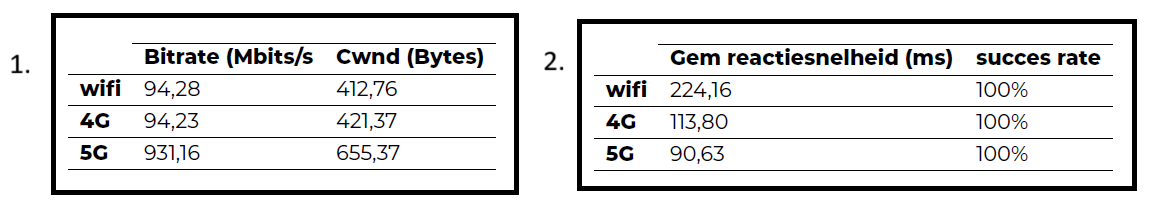
\includegraphics[width=0.45\textwidth]{../graphics/bandbreedteLicht.png}
    \captionof{figure}{Tabel 1 met de meetwaarden van de bandbreedte test en tabel 2 met de meetwaarden van de licht test}
\end{center}


\subsection*{HTTP}
De Node-RED test simuleerde periodiek HTTP-verkeer om de prestaties van wifi, 4G en 5G te vergelijken bij IoT-toepassingen. 4G presteerde het snelste en meest consistent. Wifi had de laagste doorvoersnelheid maar toonde net als 5G meer variatie. Alle netwerken waren echter voldoende snel en stabiel voor standaard IoT-gebruik zoals statusupdates en eenvoudige opdrachten.

\begin{center}
    \captionsetup{type=figure}
    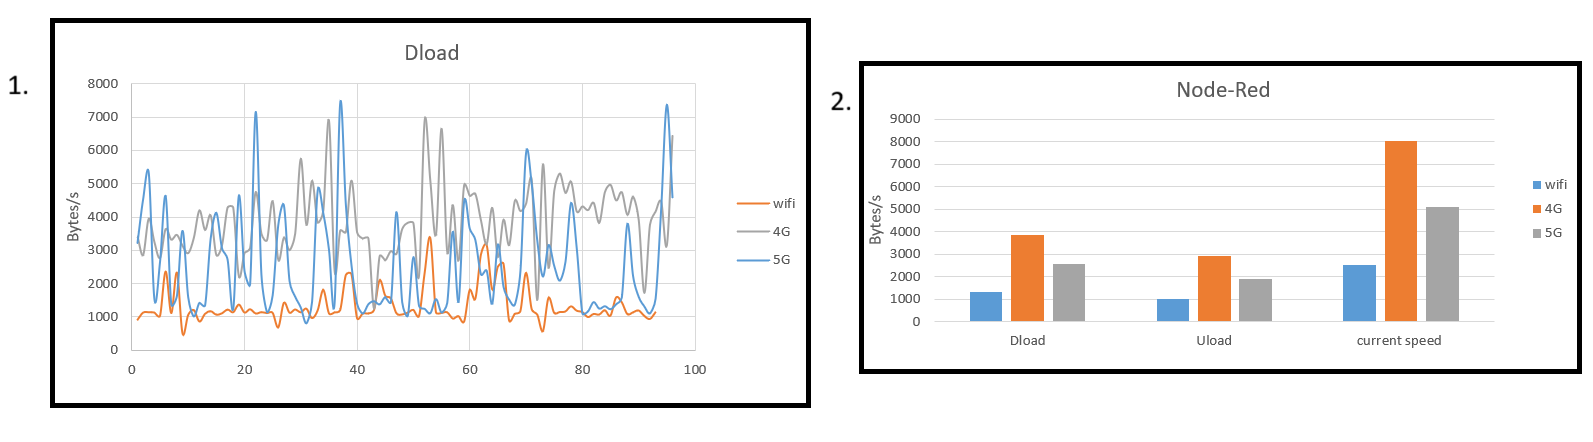
\includegraphics[width=0.45\textwidth]{../graphics/http.png}
    \captionof{figure}{Grafiek 1 is een spreidingsgrafiek van de download speed en Grafiek is de gemiddelde snelheiden van de HTTP test}
\end{center}
\section{Conclusies}
Uit de testen blijkt dat 4G de meest stabiele en betrouwbare prestaties levert, terwijl 5G uitblinkt in snelheid maar gevoelig is voor schommelingen in latency en jitter. Wifi scoorde goed qua latency, maar bleek minder betrouwbaar bij functionele opdrachten. 5G toont potentieel voor veeleisende toepassingen, mits gebruik in een gecontroleerde (private) omgeving.

\section{Toekomstig onderzoek}

Toekomstig onderzoek kan zich richten op testen binnen een private 5G-omgeving en langdurige metingen onder reële omstandigheden. Belangrijk daarbij is om ook te kijken naar schaalbaarheid, energieverbruik, roaming en beveiligingsrisico’s. Dit moet inzicht geven in de praktische inzetbaarheid van mobiele netwerken voor toepassingen van GBS. 

\end{multicols}
\end{document}